% Author: Ivan Ramos Pagnossin
% encoding: UTF-8
\documentclass{SBCbookchapter}

	\usepackage[utf8]{inputenc}
	\usepackage{ae}
	\usepackage[brazil]{babel}  
	\usepackage{graphicx}\graphicspath{{img/}}
	\usepackage{booktabs}
	\usepackage{paralist}
	\usepackage{xcolor}
	\usepackage{url}
	\usepackage{amsmath}
	\usepackage{amssymb}
	\usepackage{irpagnossin-basic}
	\usepackage{fancyhdr}
	\usepackage{calc}
	\usepackage{tikz}
	\usetikzlibrary{calc}

	\pagestyle{fancy}
	\fancyhead[L]{}
	\fancyhead[C]{}
	\fancyhead[R]{}
	\fancyfoot[L]{}
	\fancyfoot[C]{}
	\fancyfoot[R]{\thepage}
	\renewcommand{\headrulewidth}{0.0pt}

	\title{A importância da expectativa para a adoção de currículos baseados em competências em cursos livres de ciência de dados}

	\author{Ivan Ramos Pagnossin\footnote{Pós-Graduando em Computação Aplicada à Educação, USP, irpagnossin@usp.br}, S. Isotani\footnote{Seiji Isotani, USP, sisotani@icmc.usp.br}, B. E. Penteado\footnote{Bruno Elias Penteado, USP, brunopenteado@usp.br}}

	\newcommand{\campo}[1]{\ensuremath{\langle\text{#1}\rangle}}

\newenvironment{mycitation}{
	\medskip
	\noindent
	\hfill
	\begin{minipage}[t]{\textwidth-4cm}%
	\fontsize{10}{12}\selectfont%
}{
	\end{minipage}
	\medskip
}


\begin{document}
	%-- Capa
	\maketitle

	\begin{tikzpicture}[remember picture, overlay]
      \node at ($(current page.north) - (0mm,10mm)$) {
\includegraphics[width=16cm]{img/cabecalho}};
    \end{tikzpicture}
	
	\begin{resumo}
Apresentamos neste trabalho um estudo sobre como a expectativa de obter um posto de trabalho como cientista de dados afeta a aprendizagem do aluno em cursos livres de ciência de dados e promove uma situação de incompatibilidade com propostas de adoção de currículos baseados em competências.
Em vista disso propomos estratégias para contornar o problema.
Discutimos também a influência da satisfação do aluno com o curso, da relevância percebida por ele sobre os tópicos abordados e do rítmo sobre sua aprendizagem.
Mostramos que esses fatores explicam no máximo aproximadamente 20\% da aprendizagem.
\end{resumo}

\begin{abstract}
%\vspace{-0.5cm}
This work presents a study concerning how the expectancy, by the student, to achieve a work position affects his learning on courses of data science, and how this effect promotes incompatibility with proposals of adoption of competency-based curricula for these courses.
Based on that, we propose solutions to this problem.
We also argue about the influence of satisfaction with the course, perceived relevance about the topics covered by the course and the pace of his learning.
We show these factors explain, at most, approximately 20\% of student's learning.
\end{abstract}
	\vfill
	\pagebreak

	%-- Corpo
	\section{Introdução}

O interesse pela ciência de dados tem crescido nos últimos anos, assim como a quantidade de vagas de trabalho nessa área.
Consequentemente, a demanda e a oferta por cursos nessa área seguem a mesma tendência.
Porém, a definição de um currículo global de ciência de dados ainda não existe, haja vista a interdisciplinaridade dessa área.

Concomitantemente, a adoção da Educação baseada em competências como meio para desenvolver os quatro pilares da Educação do século XXI (aprender a conhecer, aprender a fazer, aprender a conviver e aprender a ser) é também um fenômeno global.
Nesse contexto, a \foreign{International Association of Business Analytics Certification} (IABAC) têm construído um arcabouço unificado e globalizado de conhecimentos, habilidades e competências para a atuação do cientista de dados.

Apesar disso, o discurso das empresas que procuram cientistas de dados no Brasil guarda uma relação explícita com conhecimentos apenas, em especial sobre ferramentas e algoritmos, sugerindo um distanciamento de qualquer proposta baseada em competências.
Isso pode dificultar, especialmente em cursos livres, o foco nas competências, pois o candidato a cientista de dados, ao confrontar os requisitos dessas vagas com as ofertas de cursos, vê mais claramente a relação com aqueles cursos que focam sua comunicação (propaganda) nesses conhecimentos.

Estamos particularmente interessados no contexto dos cursos livres, pois é nele que o primeiro autor está inserido profissionalmente.
Assim, tomamos como problema de pesquisa a adoção da aprendizagem baseada em competências em cursos livres de ciência de dados.
O objetivo geral é viabilizar essa empreitada e, para isso, começamos propondo um objetivo específico: averiguar se o fenômeno explicado no parágrafo anterior de fato existe.

Para isso, propusemos três hipóteses: a primeira delas afirma que a aprendizagem dos alunos em componentes explicitamente relacionadas com ferramentas é maior do que em componentes mais abstratas.
A segunda hipótese é similar, mas substitui ``ferramentas'' por ``algoritmos''.

A ideia subjacente a essas hipóteses é que as componentes abstratas, que são igualmente importantes para a composição de habilidades, são menos relevantes aos olhos dos alunos devido à ênfase que as ferramentas e algoritmos têm em anúncios de vagas de trabalho.

Finalmente, a terceira hipótese afirma que podemos utilizar a relevância de cada componente, conforme percebebida pelo aluno, o ritmo das aulas e a satisfação geral do aluno com o curso como preditores da aprendizagem.
Ou seja, podemos prever a aprendizagem com base nesses parâmetros.
A ideia aqui é que, se ao menos uma das duas primeiras hipóteses for verdadeira, podemos esperar alguma correlação com a relevância de cada componente, conforme percebida pelo aluno, e avaliar sua importância em comparação com o ritmo do curso e a satisfação geral do aluno.
Isso porque, mesmo que haja o efeito esperado, sua magnitude pode ser desprezível quando comparada com outros fatores.

Nós testamos essas hipóteses por meio de análise quantitativa sobre as respostas a pesquisas de levantamento apresentados aos alunos no final de cada aula.
Começamos aprofundando o cenário apresentado nos parágrafos anteriores: primeiramente, abordamos a evolução da ciência de dados e da demanda por postos de trabalho e cursos nessa área (Seção~\ref{sec:ds}).
Em seguida, voltamos nossa atenção para Educação baseada em competências e sua influência em propostas globalizadas de currículos de ciência de dados (Seção~\ref{sec:hc}).
Depois, apresentamos detalhes do cenário de aplicação deste trabalho e a motivação para ele (Seção~\ref{sec:motivacao}).
Seguimos com as referências teóricas (Seção~\ref{sec:referencial-teorico}), detalhes da metodologia de desenvolvimento deste trabalho e anállise (Seção~\ref{sec:metodologia}) para, então, apresentarmos e discutirmos os resultados (Seção~\ref{sec:resultados}).
Concluimos (Seção~\ref{sec:conclusao}) resumindo os resultados, enfatizando as limitações a apresentando possíveis prosseguimentos.
	\section{Ciência de dados}\label{sec:ds}

De acordo com o \foreign{National Institute of Standards and Technology} (NIST), ciência de dados (\foreign{data science}, DS) refere-se à atividade de extrair conhecimento acionável de conjuntos de dados brutos utilizando processos de exploração ou formulação e teste de hipóteses \cite[p.~7]{NBDIF2015}.
Ela incorpora princípios, técnicas e métodos de diversas áreas, como ciências da computação, matemática e estatística, além de domínio da área de aplicação.

Essa área tem ganhado notorieade desde o início deste século devido ao crescimento exponencial na geração de dados, conhecido genericamente como \foreign{Big Data}, devido principalmente ao advento da Web 2.0, por volta de 2005, e dos dispositivos móveis, em 2007.
Desde então e também devido ao aumento na capacidade computacional, novas técnicas de análise, a maioria computacionais, tem sido empregadas.
Exemplos notáveis são as redes neurais e a inferência bayesiana.

Nos últimos anos, inúmeras ferramentas robustas de computação e análise de dados, disponibilizadas livremente, têm tornado a ciência de dados cada vez mais acessível \cite{Hayes2019}.
Exemplos são as linguagens de programação Scala \cite{Bugnion2016}, Python \cite{Nagpal2019}, R \cite{James2013} e, mais recentemente, Julia \cite{McNicholas2019}.
Isso sem mencionar a abordagem AutoML, que oferece interfaces simples para o emprego de aprendizagem de máquina sem a necessidade de programação \cite{He2020}.

A facilidade de acesso e a alta demanda por cientistas de dados levou, então, à oferta de cursos de ciência de dados \cite{Hassan2019}: no Brasil, algumas universidades, como a Univesp, a USP e a FIAP, já oferecem cursos de graduação e pós-graduação.
Mas também é possível estudar gratuitamente pela Internet, nas plataformas MOOC (\foreign{Massive Open Online Courses}) como Coursera (\url{coursera.org}), EdX (\url{edx.org}) \etc.

Há também cursos livres nessa área, que ganham força devido ao reconhecimento de que as universidades tradicionais já não suprem a necessidade de mão de obra qualificada em várias áreas \cite{Zulauf2006}.
Esses cursos oferecem uma formação rápida, que varia em torno de um semestre, e visam colocar o candidato no mercado de trabalho independentemente da sua área de formação.
Consulte, por exemplo, os cursos de \foreign{Data Analytics} e \foreign{Data Science} da Digital House (\url{digitalhouse.com/br}) e da Tera (\url{somostera.com}).

\begin{figure}
	\centering

	
\includegraphics[width=0.45\textwidth]{eg_ds_1}\hfill
	
\includegraphics[width=0.45\textwidth]{eg_ds_2}

	\caption{Anúncios de cursos livres de ciência de dados.}
	\label{fig:cursos}
\end{figure}

Porém, como esses cursos visam o mercado de trabalho, em geral a divulgação deles enfatiza não os conhecimentos, competências e habilidades que um cientista de dados precisa, mas sim as ferramentas e algoritmos utilizados por eles e que são frequentemente mencionados em vagas de de emprego.

A Figura~\ref{fig:cursos} ilustra isso: ela apresenta a propaganda de dois cursos, oferecidos na rede social Instagram.
Em ambos o foco é linguagens de programação (Python, Scala e R), ferramentas de \foreign{Big Data} (Spark, Hadoop \etc), aplicativos (Tableau) e bibliotecas (Pandas, SciPy \etc).

Embora o domínio dessas ferramentas seja necessário, ele não é suficiente para um cientista de dados de fato produzir conhecimento acionável.
Para isso são necessários, por exemplo, métodos de pesquisa, engenharia de dados, inferência estatística, dentre outros \cite[p.~15]{CF-DS-Release2019}.

Argumentamos, então, que a ênfase em ferramentas, linguagens \etc na \emph{divulgação} desses cursos esmorece, aos olhos dos alunos, a importância das habilidades e competências, haja vista que sua relação com as vagas de emprego não são tão explícitas como as linguages e ferramentas.
	\section{Competências e habilidades}\label{sec:hc}

No Brasil e no mundo, a proposta de substituir os currículos tradicionalmente baseados em conteúdo por aqueles baseados em competências e habilidades tem ganhado força.
Por exemplo, no Brasil a Base Nacional Comum Curricular (BNCC) \cite{BNCC}, homologada em 2018, ``estabelece conhecimentos, competências e habilidades que se espera que todos os estudantes desenvolvam ao longo da escolaridade básica''.

Essa abordagem tem sido adotada no ensino básico \cite{Avila2017} e superior.
De fato, ela visa a empregabilidade \cite{Butova2015}, que é também o objetivo dos cursos livres anteriormente mencionados.

Por exemplo, segundo o \foreign{EDISON Data Science Framework}, algumas competências de um cientista de dados são \cite{CF-DS-Release2019}:
\begin{compactitem}
	\item ``Usar de engenharia (geral e de software) para pesquisar, projetar, desenvolver e implementar novos instrumentos e aplicações para a coleta de dados, armazenamento, análise e visualização''.
	\item ``Utilizar eficientemente uma variedade de técnicas de análise de dados, como aprendizagem de máquina, mineração de dados, análises prescritivas e preditivas, para análise complexa de dados durante todo o ciclo de vida dos dados''
\end{compactitem}

Ademais, exemplos de habilidades são:
\begin{compactitem}
	\item ``Usar aprendizagem de máquina, tecnologia, algoritmos e ferramentas''
	\item ``Projetar experimentos, desenvolver e implementar processos de coleta de dados''
\end{compactitem}

Entretanto, as empresas frequentemente listam ferramentas e algoritmos como requisitos às vagas de trabalho que publicam, ao invés das competências e habilidades necessárias para o exercício da ciência de dados.
A Figura~\ref{fig:vagas} ilustra duas vagas dessa área, obtidas na plataforma LinkedIn.
Nela podemos ver a menção às mesmas ferramentas e algoritmos oferecidos pelos cursos livres.

\begin{figure}
	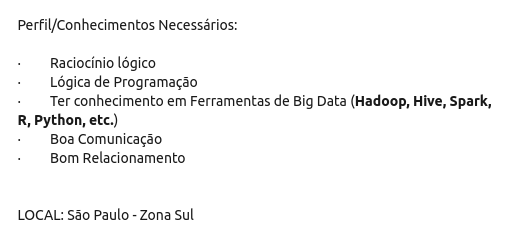
\includegraphics[width=0.45\textwidth]{eg_vaga-1_ds}\hfill
	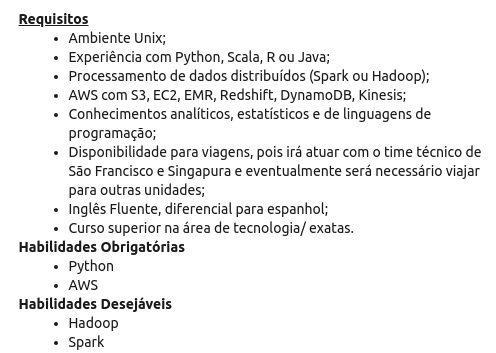
\includegraphics[width=0.45\textwidth]{eg_vaga-2_ds}
	\caption{Duas vagas de cientista de dados, extraídas do LinkedIn.}
	\label{fig:vagas}
\end{figure}
	\section{Cenário e motivação}\label{sec:motivacao}

Em vista do exposto, o autor deste trabalho, que atua como coordenador na instituição educacional Digital House (\url{digitalhouse.com/br}), que por sua vez oferece cursos livres de DS e \foreign{Data Analytics} (DA), gostaria de adotar a aprendizagem baseada em competências nos cursos de ciência de dados e de \foreign{Data Analytics} (DA) sob sua responsabilidade.

Neste trabalho nós analisamos os resultados de aprendizagem nos cursos de DA e DS oferecidos pela instituição educacional mencionada, com o intuito de identificar uma possível concorrência entre os currículos baseados em competências e os incentivos do mercado de trabalho, conforme exposto nas hipóteses deste trabalho (Seção~\ref{sec:hipoteses}).

Conforme a definição de ciência de dados do NIST, os cursos de DA e DS podem ser classificados como de ciência de dados.
Porém, eles guardam semelhanças e diferenças entre si:
\begin{compactitem}
	\item \textbf{\foreign{Data Analytics} (DA):} visa a inteligência de mercado (\foreign{Business Intelligence}, BI), isto é, a aplicação da ciência de dados para obter conhecimento acionável que suporte decisões estratégicas para um empreendimento.
	Esse curso tem carga horária de 140 horas e dura 14 semanas.
	Outra característica desse curso é que ele baseia-se em aplicativos como PowerBI, Tableau, MySQL \etc.

	\item \textbf{\foreign{Data Science} (DS):} visa o desenvolvimento de ``produtos de dados'', isto é, \foreign{softwares} que automaticamente obtém conhecimento acionável para oferecê-lo aos clientes.
	Esse curso tem carga horária de 196 horas, dura 19 semanas e baseia-se na linguagem de programação Python e suas extensões para análise de dados.
\end{compactitem}

A Tabela~\ref{tab:da-vs-ds} resume o que foi exposto imediatamente acima, comparando os dois cursos.
Note que, atualmente, os cursos em questão \emph{não} são baseados em competências.
De fato, esse é nosso objetivo geral.

\begin{table}
	\caption{Comparação dos cursos de DA e DS.}
	\label{tab:da-vs-ds}
	\footnotesize
	\begin{tabular}{lllll}
		\toprule
		Curso & Objetivo & \shortstack[l]{Carga\\horária (horas)} & \shortstack[c]{Duração\\(semanas)} & Ferramenta\\
		\midrule
		DA & Inteligência de mercado & 140 & 14 & Aplicativos (\eg, PowerBI)\\
		DS & Produto de dados & 196 & 19 & Linguagem de programação (\eg, Python)	\\
		\bottomrule
	\end{tabular}
\end{table}
	\section{Referencial teórico}

Nesta seção apresentamos as referências teóricas que suportam o desenvolvimento deste trabalho: começamos abordando a aprendizagem baseada em competências ({Seção~\ref{sec:competencias}}), com o intuito de justificar sua escolha como base para propostas de cursos de ciência de dados.
Em seguida, tratamos da teoria do valor da expectativa (Seção~\ref{sec:tve}), que utilizamos para conjecturar a razão pela qual observamos os resultados deste trabalho (Seção~\ref{sec:resultados}).
Finalmente, mencionamos a aprendizagem significativa (Seção~\ref{sec:as}) pois, conforme nossas conclusões, pode ser utilizada para intervir num dos resultados observados.

\subsection{Aprendizagem baseada em competências}
\label{sec:competencias}

Uma competência é uma coleção de habilidades e conhecimentos para realizar uma tarefa \cite{Voorhees2001}.
Alternativamente, a BNCC \cite{BNCC} define competência como ``a mobilização de conhecimentos (conceitos e procedimentos), habilidades (práticas, cognitivas e socioemocionais), atitudes e valores para resolver demandas complexas da vida cotidiana, do pleno exercício da cidadania e do mundo do trabalho''.

A aprendizagem baseada em competências é aquela que define objetivos de aprendizagem em termos dessas competências, que devem ser mensuráveis.
Isto é, ``se uma proposta de competência não puder ser descrita sem ambiguidade ou ser medida, provavelmente não é uma competência'' \cite{Voorhees2001}.

No Brasil a adoção dessa metodologia no Ensino Básico foi oficializada por meio da BNCC, aprovada em 2017, que define os conhecimentos, competências e habilidades mínimos que todos os cidadãos brasileiros devem desenvolver antes do Ensino Superior.

Embora a BNCC limite-se à Educação Básica, existe a preocupação de utilizar também essa abordagem no Ensino Superior, particularmente em resposta ao mercado de trabalho.
De fato, a Organização das Nações Unidas para a Educação, a Ciência e a Cultura (Unesco) já defendia as bases da Educação para o século XXI com os pilares (1) aprender a conhecer, (2) aprender a fazer, (3) aprender a conviver e (4) aprender a ser, propostos por Pirrenoud em 1970.

Realmente, esse modelo surgiu nos Estados Unidos, nos anos 1960, com o intuito de resolver a crescente disparidade entre as necessidades do mercado de trabalho e o que as universidades oferecem aos seus estudantes \cite{Zulauf2006}: 

\begin{mycitation}
	``[No] mercado e os ambientes de trabalho, o ensino superior vem sofrendo crescente pressão para desenvolver a empregabilidade dos estudantes e tornar-se mais relevante no que diz respeito às necessidades dos empregadores.''
\end{mycitation}

Embora haja inúmeras iniciativas \foreign{ad hoc} de criar um currículo para o ensino da ciência de dados \cite{Hassan2019, Anderson2014, Cheng2019}, tem surgido atualmente iniciativas de unificação \cite{Raj2019}.
Uma das que merece menção é a \foreign{EDISON Data Science Framework}, desenvolvida pela \foreign{International Association of Business Analytics Certification} (IABAC), que provê uma base para a definição da profissão de cientista de dados, bem como componentes relacionados como educação, treinamento, papéis, dentre outros.
Ela define três especificações:
\begin{compactitem}
	\item \foreign{Data Science Competence Framework} (CF-DS) é o núcleo da especificação, que inclui as competências necessárias para o cientista de dados atuar no mercado de trabalho e na academia ao longo de toda sua carreira.
	\item \foreign{Data Science Body of Knowledge} (DS-BoK) define áreas de conhecimento para a construção de currículos de ciência de dados que comportem as competências identificadas no CF-DS \cite{Demchenko2017}.
	\item \foreign{Data Science Model Curriculum} (MC-DS) define objetivos de aprendizagem consonantes com a CF-DS e unidades de aprendizagem associadas às unidades de conhecimento definidas no DS-BoK.
\end{compactitem}

Assim, defendemos que os currículos de cursos de ciência de dados devam ser baseados em competências e habilidades.
Porém, o mercado impõe dificuldade a essa empreitada pois, ao enfatizar ferramentas nas vagas de emprego, incentiva o candidato a cientista de dados a procurar cursos que lhe deem esse \emph{conhecimento}.
Procuramos fundamentar essa suposição com base na teoria do valor da expectativa, na próxima seção.

\subsection{Teoria do valor da expectativa}\label{sec:tve}
%\cite{Wigfield2000}
%\cite{Guo2015}?

% iedunote.com/expentancey-theory
Em 1964, Victor H. Vroom desenvolveu a sua teoria comportamentalista do valor da expectativa \cite{Petri}, uma teoria da motivação, segundo a qual ``a escolha, persistência e desempenho de indivíduos pode ser explicada por sua crença sobre quão bem ele executará uma atividade e quanto ele valoriza essa atividade''.
A teoria propõe ainda que a motivação depende de três fatores: 
\begin{compactitem}
	\item Resultado ou recompensa esperado, chamado de valência;
	\item Percepção de intensidade da relação entre o desempenho requerido e o resultado (instrumentalidade);
	\item Percepção do vínculo existente entre o esforço requerido e o desempenho subsequente (expectativa).
\end{compactitem}

Conforme demonstraremos nos resultados deste trabalho (Seção~\ref{sec:resultados}), a aprendizagem percebida pelo aluno em aulas explicitamente relacionadas com ferramentas é maior, dentro de um nível de significância de 95\%, que aquela em outras aulas.
Aplicamos a teoria do valor da expectativa para conjecturar que essa diferença é devida a uma maior intensidade do vínculo entre as aulas de ferramentas e as vagas de emprego (valência), levando a motivação intrínseca que promove a aprendizagem nessas aulas.

Além disso, upondo verdadeira essa conjectura, podemos ainda utilizá-la para promover a aprendizagem nas demais aulas.
Para isso, propomos (1) intensificar, pelo discurso, o vínculo entre os requisitos do mercado e os objetivos das aulas, e/ou (2) desenvolver essas aulas utilizando ferramentas, se possível, o que se baseia na aprendizagem significativa, objeto da próxima seção.

\subsection{Aprendizagem significativa}\label{sec:as}

% portaldoprofessor.mec.gov.br/storage/materiais/0000012381.pdf
Aprendizagem significativa \cite{Pelizzari2002} é a concepção cognitivista de ensino e aprendizagem proposta pelo psicólogo americano David Ausubel em 1963.
O autor afirma que o fator isolado mais relevante para a aprendizagem é o conhecimento prévio do aluno.
Ou seja, a aprendizagem ocorre quando novas informações ancoram-se em conceitos ou proposições relevantes pré-existentes.

Desse modo, podemos ancorar a aprendizagem de componentes abstratas, isto é, que têm um vínculo fraco com a valência, na aprendizagem das componentes cujo vínculo é forte (nos quais verificamos maior aprendizagem percebida).


	\section{Metodologia}
\label{sec:metodologia}

Nós utilizamos mineração de dados educacionais \cite{Baker2011} para realizar análises quantitativas sobre o dados gerados pela interação contínua dos alunos com os sistemas de informação da instituição educacional.
Ou seja, os dados aqui utilizados não foram produzidos em resposta a uma pesquisa previamente planejada.
É importante ter isso em mente porque algumas das limitações deste trabalho decorrem disso.


\subsection{Coleta dos dados}

No final de cada uma das aulas dos cursos de DA e DS, os professores divulgaram aos alunos, diretamente e pelo canal de comunicações da turma (grupo do Whatsapp), o link para um formulário do Google Forms único para aquela aula (seção~\ref{sec:formularios}).
Os alunos eram incentivados a responder, sem supervisão nem obrigatoriedade.

Os formulários foram aplicados entre 8/abr e 7/dez/2019 em 6 turmas de DA e 4 turmas de DS, totalizando até 255 alunos e gerando 1878 observações para DA e 1763 para DS.

\subsection{Formulários}
\label{sec:formularios}

Cada formulário apresentava as seguintes questões:

\begin{compactenum}
	\item Email
	
	\item Nome
	
	\item\label{q:antes} ``\campo{Área}: quanto você já sabia sobre \campo{tópico}?''.
	Escala Likert de 1 a 5.
	Chamaremos essa variável de $q_\text{antes}$ para referência futura.
	
	\item\label{q:depois} ``\campo{Área}: E agora depois da aula quanto você sabe sobre \campo{tópico}?''.
	Escala Likert de 1 a 5.
	Chamaremos essa variável de $q_\text{depois}$.
	
	\item\label{q:relevancia} ``Relevância: O quanto você acha que o conteúdo abordado é relevante para a sua formação?''. Escala Likert de 1 (``pouco relevante'') a 5 (``muito relevante'').
	
	\item\label{q:ritmo} ``Ritmo: Como você classifica o ritmo da aula de hoje?''. Escala Likert de 1 (``muito lento'') a 5 (``muito rápido'').
	
	\item\label{q:satisfação} ``Satisfação: O quanto você está satisfeit@ com a aula de hoje?''.
	Escala Likert de 1 (``pouco satisfeit@'') a 10 (``muito satisfeit@'')
	
	\item ``Se quiser fornecer algum feedback ou comentário específico use o espaço abaixo (não obrigatório)''.
	Discursiva.
	Não utilizada neste trabalho.
\end{compactenum}

As questões~\ref{q:antes} e \ref{q:depois} podem ser repetidas até 4 vezes (ou seja, cada aula pode apresentar até 4 tópicos), em que \campo{Área} representa a macro-componente do curso (tecnologia, negócios ou estatística) e \campo{tópico} é um texto escrito livremente pelo professor, que aborda um tópico da aula.
Exemplos de \campo{tópico} são: ``Aplicabilidade da regressão logística'', ``Fundamentos do MySQL'' \etc (ao todo são 985 valores distintos no conjunto de dados original).

\subsection{Variáveis}

A variável-alvo (dependente) deste trabalho é a aprendizagem, cuja medida operacional $a$ foi definida como o valor numérico da questão \ref{q:depois} subtraído do da questão \ref{q:antes}:
\begin{equation}\label{eq:a}
	a := q_\text{depois} - q_\text{antes}
\end{equation}

Por exemplo, se o aluno respondeu $q_\text{antes} = 2$ para a questão \ref{q:antes} (quanto ``sabe'' antes da aula) e $q_\text{depois} = 5$ para a questão \ref{q:depois} (depois), então a aprendizagem foi de $a = 5 - 2 = 3$.
Desse modo, essa variável assume valores inteiros no intervalo $[-4,4]$ e, conforme \cite{Harpe2015}, pode ser interpretada como numérica.

As variáveis independentes são:
\begin{compactitem}
	\item Relevância (questão \ref{q:relevancia}).
	Variável categórica com cardinalidade 5.

	\item Rítmo (\ref{q:ritmo}).
	Variável categórica com cardinalidade 5.

	\item Satisfação (\ref{q:satisfação}).
	Variável numérica discreta.

	\item \campo{tópico}.
	Variável categórica (texto) com cardinalidade 985.
\end{compactitem}

A natureza de cada variável acima (numérica ou categórica) foi decidida com base nas recomendações de \cite{Harpe2015}.

\section{Conjunto de dados}

A análise e resultados deste trabalho foram desenvolvidos a partir de um conjunto de dados armazenado num arquivo no formato CSV (\foreign{comma-separated values}).
Esse arquivo, por sua vez, foi construído aglomerando as respostas dos alunos aos inúmeros formulários aplicados, um por aula, turma e curso, utilizando a linguagem de \foreign{script} Google Apps Script.

Os dados originais contêm identificação dos alunos e, por isso, o arquivo disponibilizado para reprodutibilidade deste trabalho (apêncie~\ref{ap:rr}) passou por uma etapa de preprocessamento em que apenas removemos a identificação dos alunos, trocando por ``Aluno 1'', ``Aluno 2'' \etc.

\section{Ferramentas de análise}

A análise foi realizada utilizando \foreign{softwares} gratuitos: Python 3.8 com a interface JupyterLab e as bibliotecas Pandas (manipulação de dados), statsmodel (modelagem estatística), scikit-learn (\foreign{machine learning}), dentre outras.

	\section{Resultados e discussão}
\label{sec:resultados}

	\subsection{Pré-processamento}
\label{sec:pre-processamento}

A primeira etapa na análise de dados foi transformar o arquivo dos dados para o padrão \foreign{tidy-data} \cite{Wicham2014}, onde cada linha representa a resposta de um aluno para cada um dos até 4 tópicos abordados numa aula.
A Tabela~\ref{tab:dataset-raw} ilustra as primeiras linhas desse arquivo.

\begin{table}
	\centering
	\caption{As primeiras linhas do conjunto de dados utilizados neste trabalho.}
	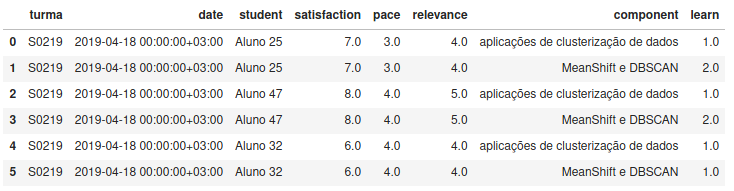
\includegraphics[width=\textwidth]{tidy-sample}
	\label{tab:dataset-raw}
\end{table}

Note que as duas primeiras linhas representam as respostas do ``Aluno 25'' ao formulário aplicado na aula de 18/abr/2019 da turma S2019. Nessa aula dois tópicos foram abordados: ``aplicações de clusterização de dados'' e ``MeanShift e DBSCAN''. No primeiro deles a aprendizagem foi de 1 unidade (última coluna) e, no segundo, de 2 unidades.

Em vista de cada formulário poder apresentar até quatro tópicos (dois neste exemplo), as informações de satisfação (\foreign{satisfaction}), ritmo (\foreign{pace}) e relevância (\foreign{relevance}) estão duplicados. Isso significa que, ao analisarmos essas variáveis, precisamos remover essas duplicidades.
Fizemos isso através de uma amostragem que selecionava, aleatoriamente, \emph{uma} linha para cada tupla (curso, turma, aula, aluno).
Por exemplo, se selecionássemos a primeira linha, certamente ignoraríamos a segunda linha.

Esse arquivo foi posteriormente transformado:
\begin{compactitem}
	\item Criamos uma coluna para identificar o curso (\foreign{course}), com valores DA ou DS, a partir da turma: aquelas que iniciam com ``A'' são de DA; as com ``S'', são DS.
	
	\item A turma foi trocada por um valor numérico sequencial arbitrário.
	
	\item As colunas de satisfação, ritmo e relevância foram normalizadas no intervalo $[0,10]$, apenas por simplicidade.

	\item Criamos a coluna \foreign{component}, que mapeia o tópico para uma hierarquia \foreign{ad-hoc} de componentes de cada curso.
	Por exemplo, o tópico ``Construção e execução de queries'' foi mapeado para o componente ``SQL/\textbf{Ferramenta}'' (DA), enquanto ``ARIMA. SARIMAX e Prophet'' foi mapeado para ``Séries temporais/\textbf{Algoritmo}'' (DS).
	O mapeamento foi feito manualmente para os 985 tópicos presentes.

	\item Criamos a coluna \foreign{tool}, variável categórica booleana, para indicar se a aula contém algum componente de ferramenta.
	Isso foi feito a partir da coluna \foreign{component}: se ela contém ``Ferramenta'', então o valor dessa variável é ``verdadeiro''; se não, é ``falso'' (veja grifos no item anterior).
	
	\item Criamos a coluna \foreign{algorithm}, variável categórica booleana, para indicar se a aula contém algum componente de algoritmo.
	Isso foi feito de maneira similar ao item anterior, também a partir da coluna \foreign{component}.
\end{compactitem}

A Tabela~\ref{fig:dataset} ilustra o conjunto de dados após esse pré-processamento e já pronto para a análise.

\begin{table}
	\centering
	\caption{O conjunto de dados, pronto para a análise.}
	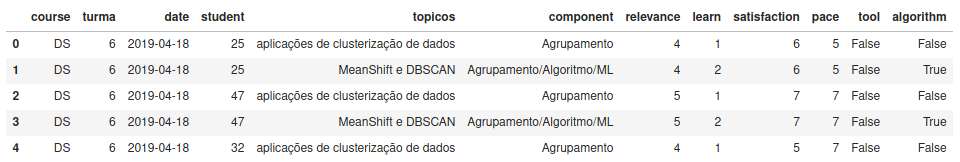
\includegraphics[width=\textwidth]{tidy-sample-2}
	\label{fig:dataset}
\end{table}
	\subsection{Hipótese 1}
\label{sec:resultados-hipotese-1}

Primeiramente vamos avaliar a hipótese 1.
Nesse caso, queremos avaliar a variável dependente $a$, isto é, a aprendizagem; coluna \foreign{learn} na Tabela~\ref{fig:dataset}.
A estratégia é simples: para cada um dos cursos (DA e DS), vamos segmentar o conjunto de dados em dois sub-conjuntos, um das aulas referentes a ferramentas; o outro com o complemento deste (demais aulas).
Em seguida, aplicamos um teste de hipótese estatístico para avaliar a hipótese nula de que a média $\mu_f$ da aprendizagem da população de todas as aulas referentes a \textbf{f}erramentas é igual à média $\mu_{\neg f}$ da aprendizagem da população das demais aulas.
Ou seja,
\begin{align*}
	H_0&: \mu_f = \mu_{\neg f} \\
	H_a&: \mu_f > \mu_{\neg f}
\end{align*}

O conjunto de dados pré-processado já contém a informação de que um dado componente refere-se a uma ferramenta ou não (coluna \foreign{tool} na Figura~\ref{fig:dataset}).
Assim, podemos segregar o conjunto de dados segundo esse critério.

\begin{figure}[b]
	\centering
	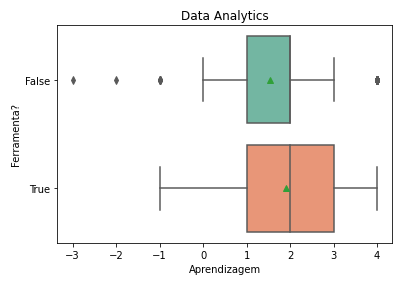
\includegraphics[width=0.45\textwidth]{da-boxplot-by-tool}\hfill
	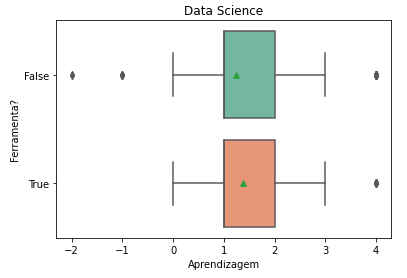
\includegraphics[width=0.45\textwidth]{ds-boxplot-by-tool}
	\caption{Distribuição da aprendizagem nos cursos de DA (esquerda) e DS (direita) para as aulas de ferramentas (\foreign{true} no eixo vertical) e as demais. Os triângulos verdes indicam a média amostral.}
	\label{fig:dist-hipotese-1}
\end{figure}

Note que a hipótese 1 baseia-se na suposição de que podemos calcular a média das aprendizagens.
Há décadas discute-se sobre a possibilidade de interpretar a escala Likert como variável numérica.
Considerando que os valores de $q_\text{antes}$ (idem para $q_\text{depois}$) guardam entre si uma relação de ordenação, a partir da qual é possível construir um espaço métrico \cite[cap.~27]{Barata2020}, mais as recomendações de \cite{Harpe2015}, consideramos válido assumir que $a$ (equação~\ref{eq:a}) é de fato numérica e que, por isso, $\mu_f$ e $\mu_{\neg f}$ existem, bem como a média de qualquer amostra dessas populações, $\bar a_f$ e $\bar a_{\neg f}$ (usamos $\bar a$ sem subscrito quando queremos fazer referência a qualquer uma das duas médias amostrais).

A Figura~\ref{fig:dist-hipotese-1} apresenta a distribuição dos valores de aprendizagem $a$ para os sub-conjuntos: \foreign{true} refere-se às aulas de ferramenta.

A Tabela~\ref{tab:dist-hipotese-1} apresenta as médias, desvio-padrão e erro-padrão da média (nível de significância de 5\%) para cada um dos sub-conjuntos dos cursos de DA e DS.
Vemos, por exemplo, que para DA a média amostral de aprendizagem nas aulas de ferramentas é de $1,9\pm{0,1}$, ou seja, ela reside no intervalo $1,8 \le \bar a_f \le 2,0$.
Note que esse intervalo \emph{não} contém a média da aprendizagem nas demais aulas, $\bar a_{\neg f}$, cujo valor máximo é de $1,6$.
Observação análoga pode ser feita para DS, à direita na tabela.
Esse resultado é um indício de que realmente há uma diferença entre as médias populacionais, mas para fazermos essa afirmação precisamos do teste t.

\begin{table}
	\caption{Tamanho da amostra (\#), média $\bar a$ (e erro padrão) e desvio-padrão $s_a$ de cada sub-conjunto de DA (esquera) e DS (direita).}
	\label{tab:dist-hipotese-1}
	\centering
	\begin{minipage}{0.45\textwidth}
		\begin{tabular}{lrrr}
			\toprule
			\multicolumn{4}{c}{Data Analytics}\\
			Ferramenta? & \# & $\bar{a}$ & $s_a$ \\
			\midrule
			Sim &  408 & $1,9\pm 0,1$ & 1,1 \\
			Não & 1470 & $1,55 \pm 0,05$ & 1,1 \\
			\bottomrule
		\end{tabular}
	\end{minipage}\hfill
	\begin{minipage}{0.45\textwidth}
		\begin{tabular}{lrrr}
			\toprule
			\multicolumn{4}{c}{Data Science}\\
			Ferramenta? & \# & $\bar{a}$ & $s_a$ \\
			\midrule
			Sim &  232 & $1,4\pm 0,1$ & 1,0 \\
			Não & 1531 & $1,23\pm 0,04$ & 0,9 \\
			\bottomrule
		\end{tabular}
	\end{minipage}
\end{table}

Antes de efetuarmos o teste da hipótese 1, vamos checar se ambos os sub-conjuntos apresentam distribuição normal.
Para isso utilizamos o teste de Lilliefors com nível de significância de 5\% (valor-padrão na literatura e não temos argumentos para usar um valor diferente).
O resultado é um valor-$p$ bastante inferior ao nível de significância, o que significa que a distribuição \emph{não} é normal.
Apesar disso, segundo~\cite[p.~259]{Triola2005} é possível realizar o teste t a seguir mesmo que a amostra não provenha de uma distribuição normal, desde que a amostra tenha tamanho maior do que 30, que é o nosso caso: o menor dos sub-conjuntos tem 232 observações.

Executamos o teste t de duas amostras independentes com populações cuja variância é desconhecida.
Para DA obtivemos $\text{valor-}p \approx 4\times10^{-8}$ com a estatística t positiva: veja a Tabela~\ref{tab:hipotese-1}.
Isso significa que a probabilidade de observarmos uma distribuição amostral com a média $\bar a = 1,9\pm 0,1$, sob a suposição de que essa amostra tem origem numa população cuja média $\mu_f = 1,55\pm 0,05$, é da ordem de $4\times10^{-8}$.
Ou seja, é improvável.
Na verdade, é mais improvável do que o que originalmente escolhemos aceitar, o nível de significância de 5\%.
Logo, podemos rejeitar $H_0$ e afirmar que nossos dados suportam a hipótese de que $\mu_{f} > \mu_{\neg f}$ para DA.

Em palavras, os alunos ``aprendem mais'' nas aulas referentes a ferramentas do que nas demais aulas de DA.


Análise análoga pode ser feita para DS (Tabela~\ref{tab:hipotese-1}): o valor $p$ é inferior ao nível de significância e a estatística t é positiva, significando que também para DS os alunos aprendem mais nas aulas referentes a ferramentas do que nas demais.

À luz da teoria do valor da expectativa, podemos argumentar que as aulas de ferramentas oferecem aos alunos uma relação explícita (instrumentalidade) com as demandas de vagas de postos de trabalho, de modo que a expectativa de obter um emprego (valência) promove no aluno motivação intrínseca para aprender.
Essa relação não é tão evidente nas demais aulas, levando a uma instrumentalidade menor e, por conseguinte, menor motivação para aprender.


\begin{table}
	\centering
	\caption{Resultado do teste da hipótese 1 nos cursos DA e DS.}
	\label{tab:hipotese-1}

	\begin{tabular}{lcc}
	\toprule
	Curso & Valor $p$   & Estatística $t$ \\
	\midrule
	DA    & $<10^{-11}$ & $7,24$ \\
	DS    & $0,03$      & $2,13$ \\ 
	\bottomrule
	\end{tabular}
\end{table}

% britannica.com/topic/motivation/Behavioristic-approaches-to-motivation
Essa aprendizagem aprimorada nas aulas de ferramentas pode ser, ainda, um efeito do chamado condicionamento operante \cite{Petri}, uma abordagem comportamentalista da motivação: a utilização das ferramentas leva a resultados concretos que, por sua vez, motivam aprendizagens subsequentes.

Independentemente do processo cognitivo, intangível à experiência, o fato é que há diferença.
Isso sugere que podemos utilizar essa motivação nas demais aulas.
Duas possibilidades nos ocorre: (1) desenvolver as demais aulas utilizando as ferramentas, se possível (aprendizagem significativa); e (2) tornando evidente, por discurso ou pela aplicação de projetos extraídos do mercado de trabalho, a relação com os requisitos do mercado (teoria do valor da expectativa).
	\subsection{Hipótese 2}

A verificação da hipótese 2 é similar à da primeira, exceto que dessa vez segmentamos os dados em aulas que envolvem explicitamente algoritmos ou não
.
Na seção~\ref{sec:resultados} nós mostramos como essas aulas foram identificadas (coluna \foreign{algorithm} do conjunto de dados), restando agora executar a segmentação e o teste t.

\begin{figure}
	\centering
	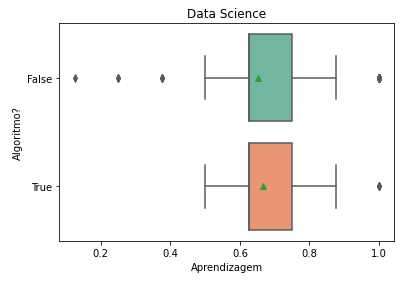
\includegraphics[width=0.45\textwidth]{ds-boxplot-by-algorithm}
	\caption{Distribuição da aprendizagem no cursos de DS para cada sub-conjunto analisado: aulas de algoritmos (\foreign{true} no eixo vertical) e as demais. Os triângulos verdes indicam a média amostral.}
	\label{fig:dist-hipotese-2}
\end{figure}

A figura~\ref{fig:dist-hipotese-2} e a tabela \ref{tab:dist-hipotese-2} apresentam a distribuição da aprendizagem das aulas de ferramentas e das demais do curso de DS.

O curso de DA não tem ênfase em algoritmos.
Por isso não propusemos fazer teste análogo nele.
De fato, podemos verificar no conjunto de dados que a quantidade de aulas com o atributo \foreign{algorithm} = \foreign{true} é zero.

Note, na tabela~\ref{tab:dist-hipotese-2}, que a média amostral das aulas de algoritmo reside no intervalo $[1,1; 1,5]$, que envolve a média amostral das demais aulas.
Além disso, os desvios-padrão são similares.
Isso evidencia que as duas amostras têm origem na mesma população.
Porém, apenas o teste t nos permitirá afirmar.

\begin{table}
	\centering
	\caption{Tamanho da amostra (\#), média (e erro padrão) e desvio-padrão das aulas de algoritmos e demais do curso de DS.}
	\label{tab:dist-hipotese-2}
	\begin{tabular}{lrrr}
		\toprule
		Algoritmo? & \# & $\bar{a}$ & $s_a$ \\
		\midrule
		Sim &  110 &  1,3(2) & 0,88 \\
		Não & 1653 & 1,25(4) & 0,88 \\
		\bottomrule
	\end{tabular}
\end{table}

\begin{table}
	\centering
	\caption{Resultado do teste t no curso de DS}
	\begin{tabular}{lcc}
	\toprule
	Curso & Valor $p$   & Estatística $t$ \\
	\midrule
	DS    & $0,41$      & $0,83$ \\ 
	\bottomrule
	\end{tabular}
\end{table}

Ao efetuarmos o teste de hipótese, obtivemos valor-$p$ de 41\%.
Ou seja, a probabilidade de observarmos a média 1,3(2) numa amostra de uma população com média 1,25(4) é de 41\%, acima do nível de significância de 5\% assumido.
Logo, podemos afirmar que as duas amostras advém da mesma população.
Consequentemente, \emph{não} há diferença de aprendizagem entre as aulas de algoritmos e as demais.
	\subsection{Hipótese 3}

Agora voltamos nossa atenção para a possível relação entre a aprendizagem e a satisfação, ritmo e relevância reportados pelos alunos.

O argumento aqui é baseado na aprendizagem individualizada: o ritmo, que pode ser completamente controlado pelo aluno nessa abordagem, oferece vantagem para a aprendizagem.
E como temos informações extras sobre a satisfação e a relevância, vamos considerá-las também como critérios de comparação.

Como a aprendizagem $a$ é uma variável numérica, temos em mãos um problema de regressão.
Argumentamos que uma abordagem classificatória também é possível, desde que se tome o cuidado de garantir a integridade do espaço amostral de $a$, o intervalo $[-4,4]$.
Porém isso ficará para trabalhos futuros.

\begin{figure}[t]
	\centering

	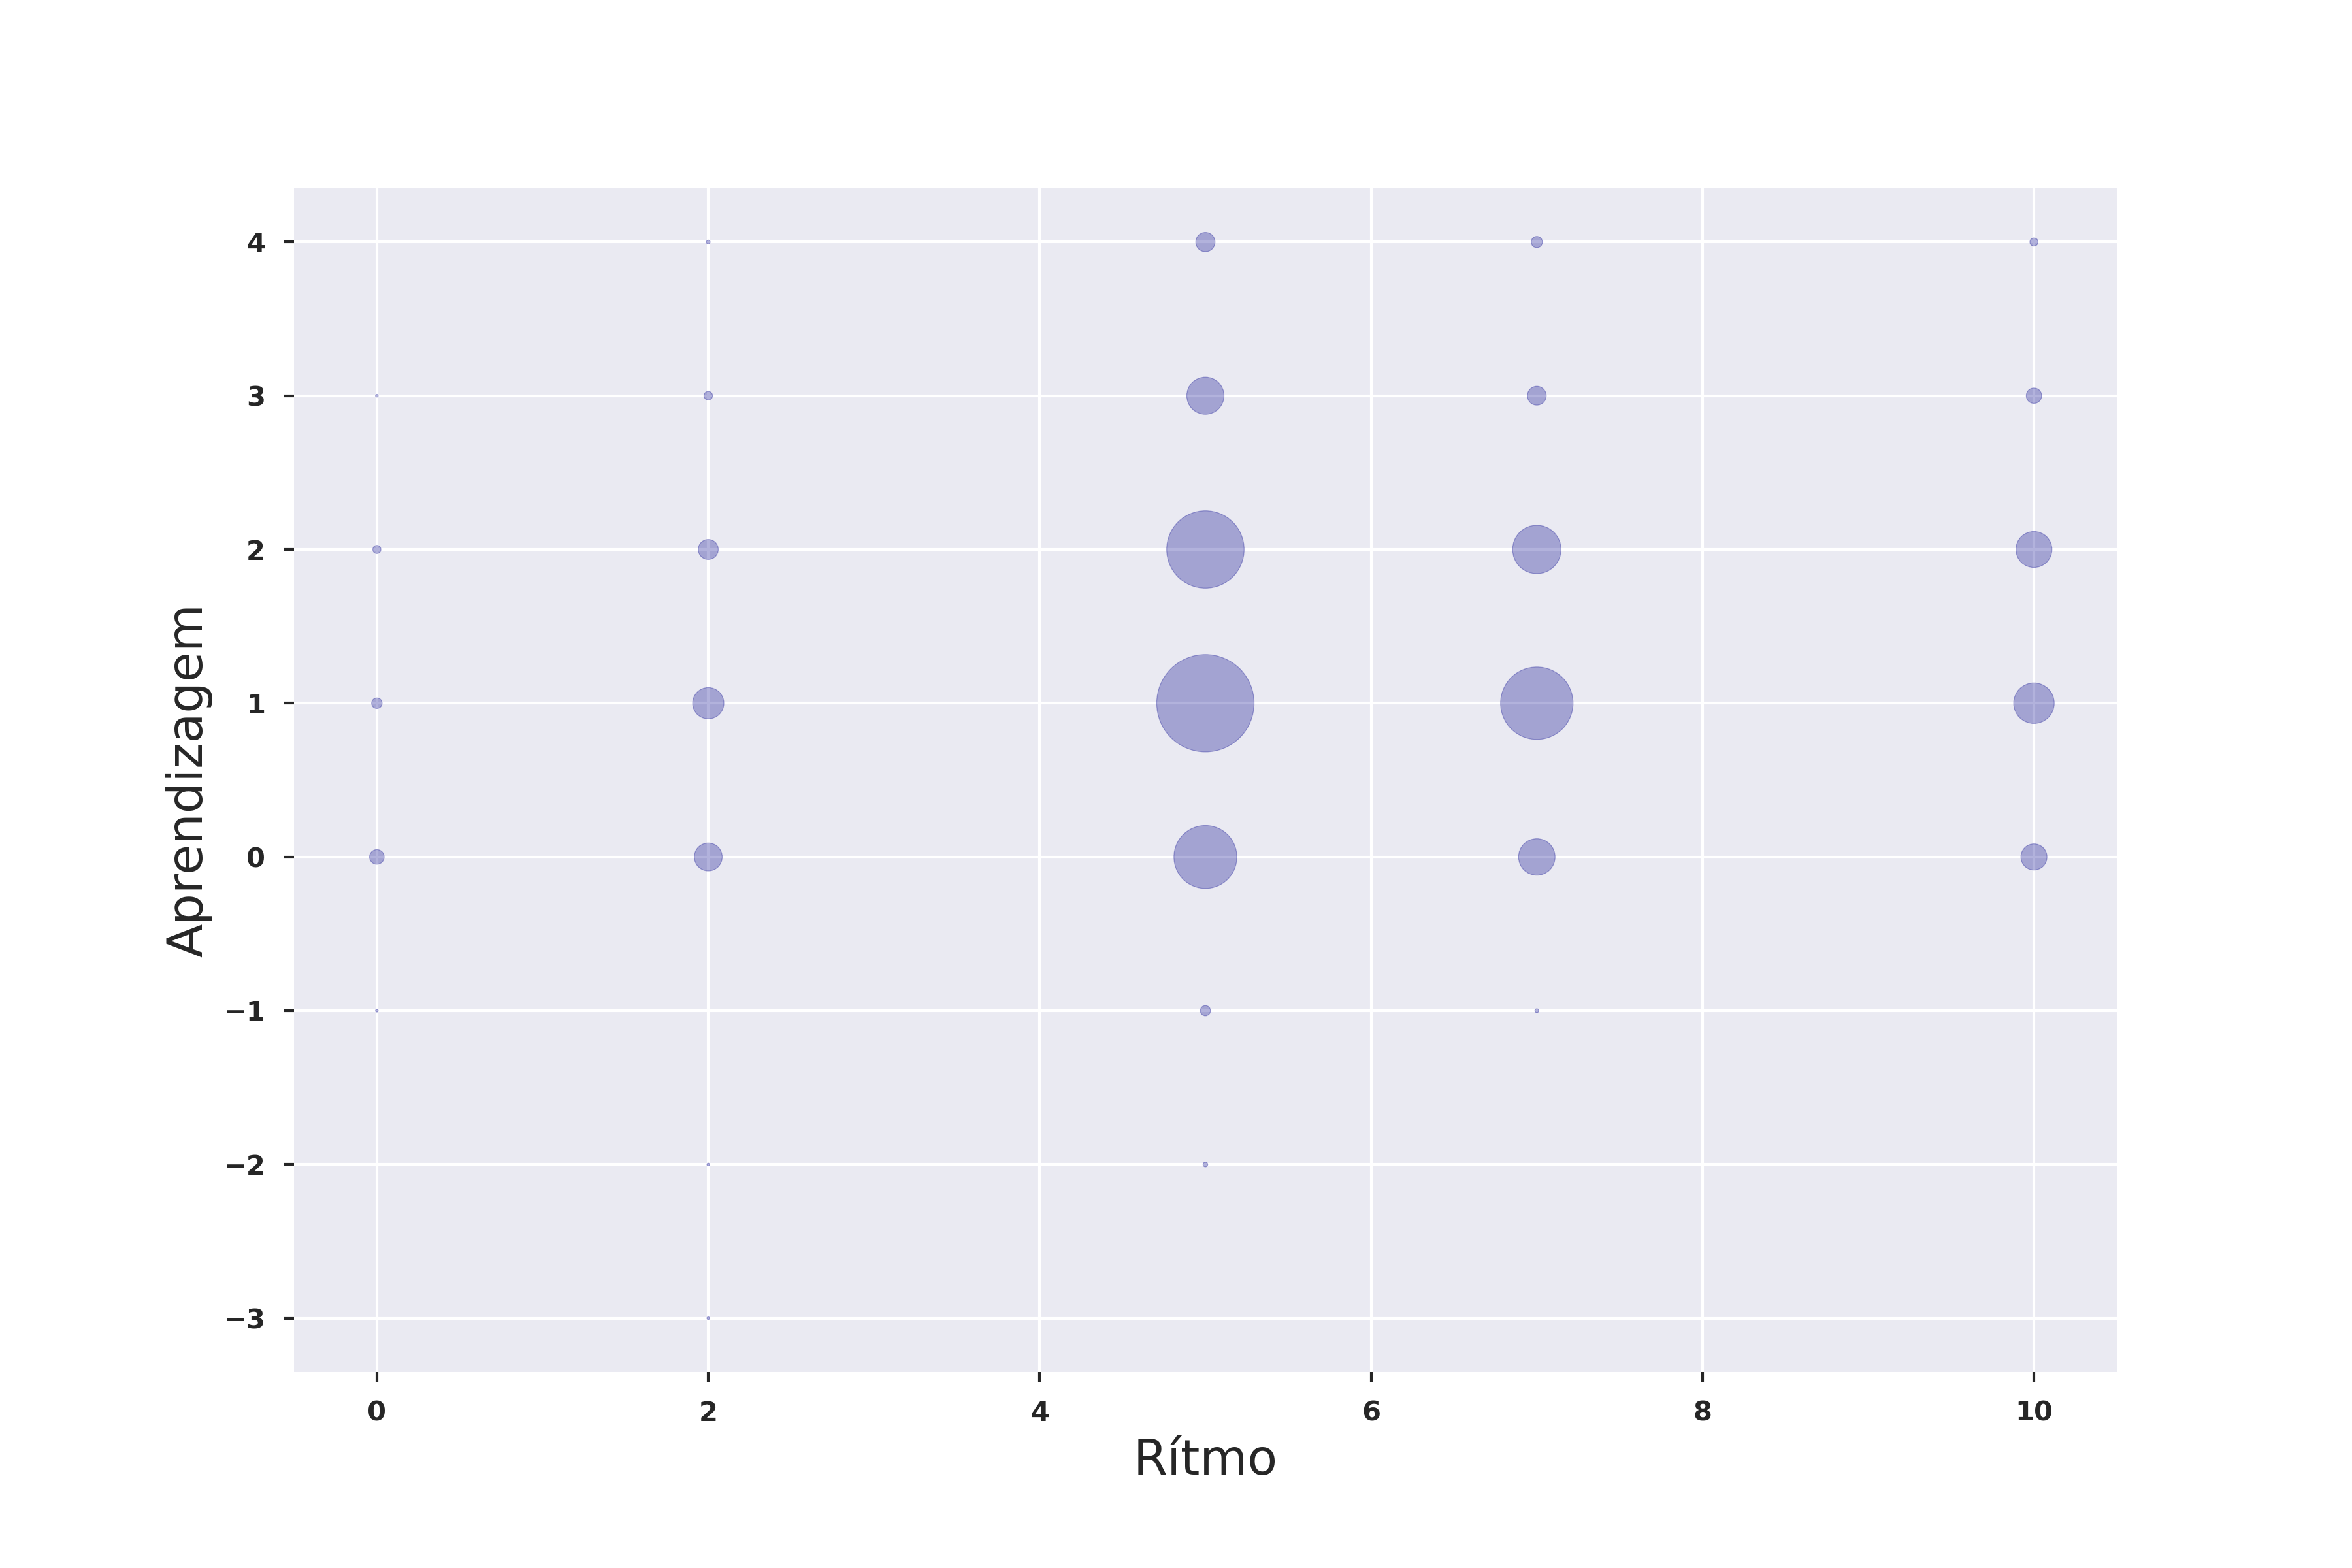
\includegraphics[width=0.5\textwidth]{aprendizagem-vs-ritmo}

	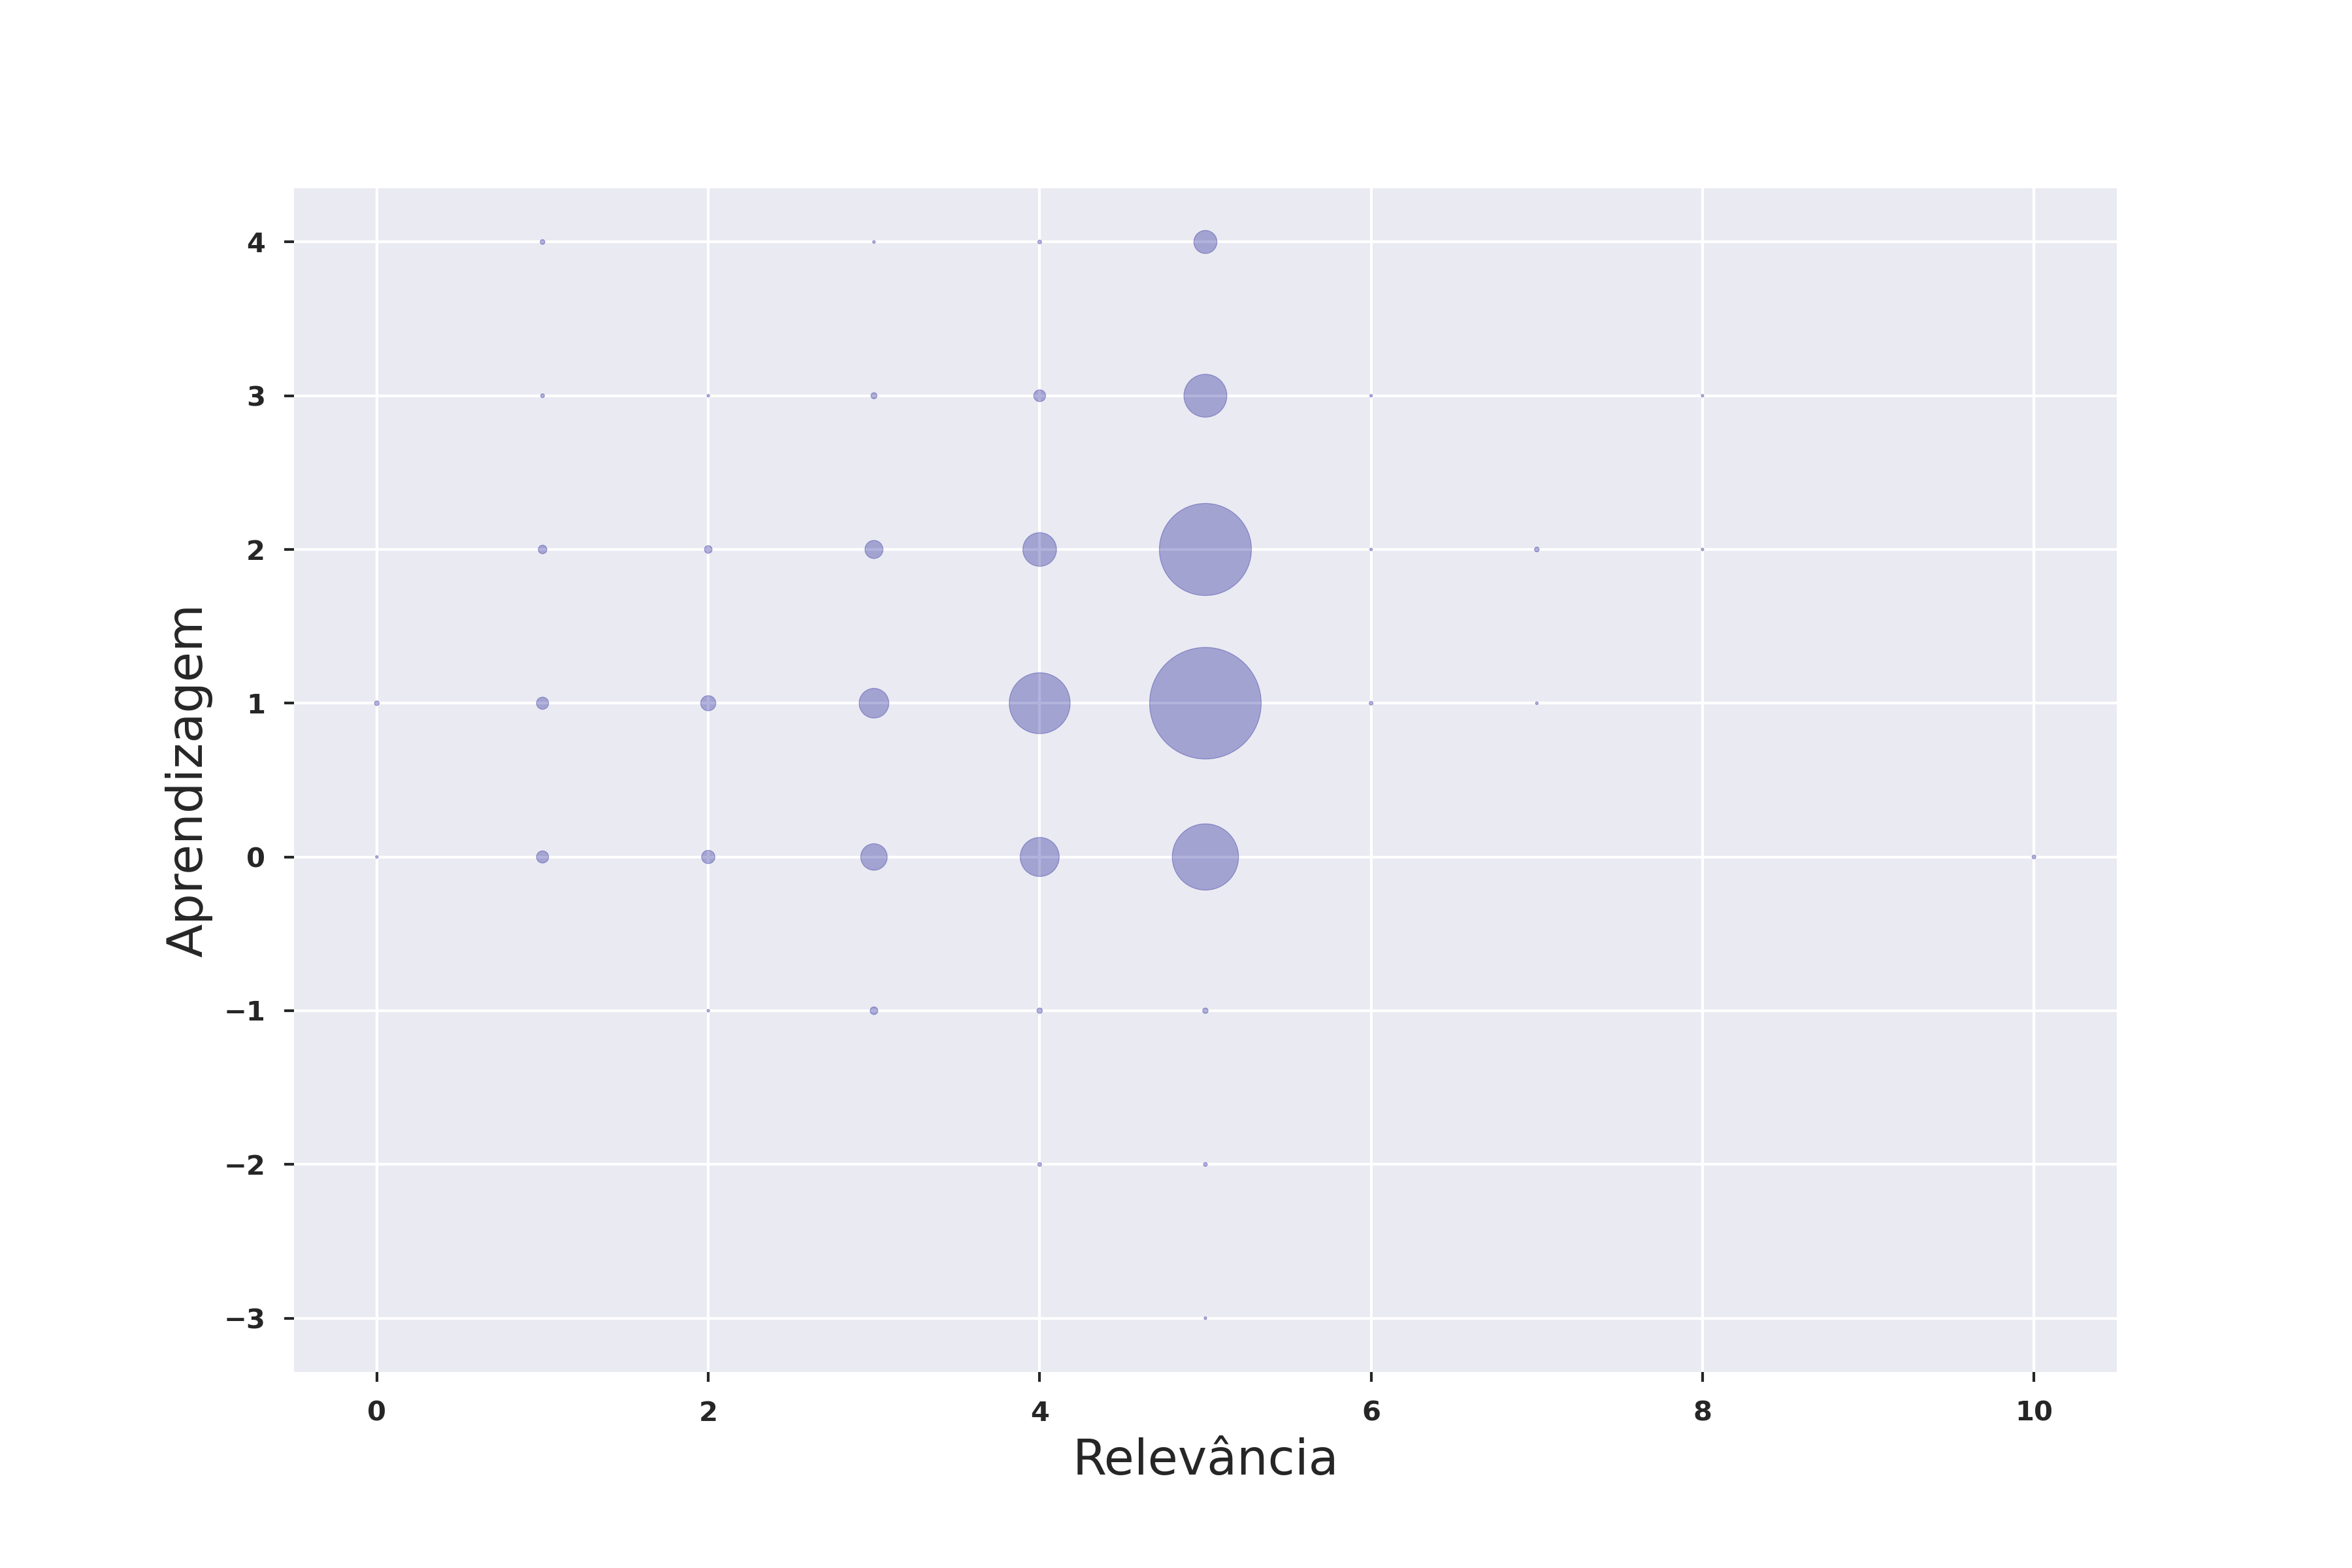
\includegraphics[width=0.5\textwidth]{aprendizagem-vs-relevancia}

	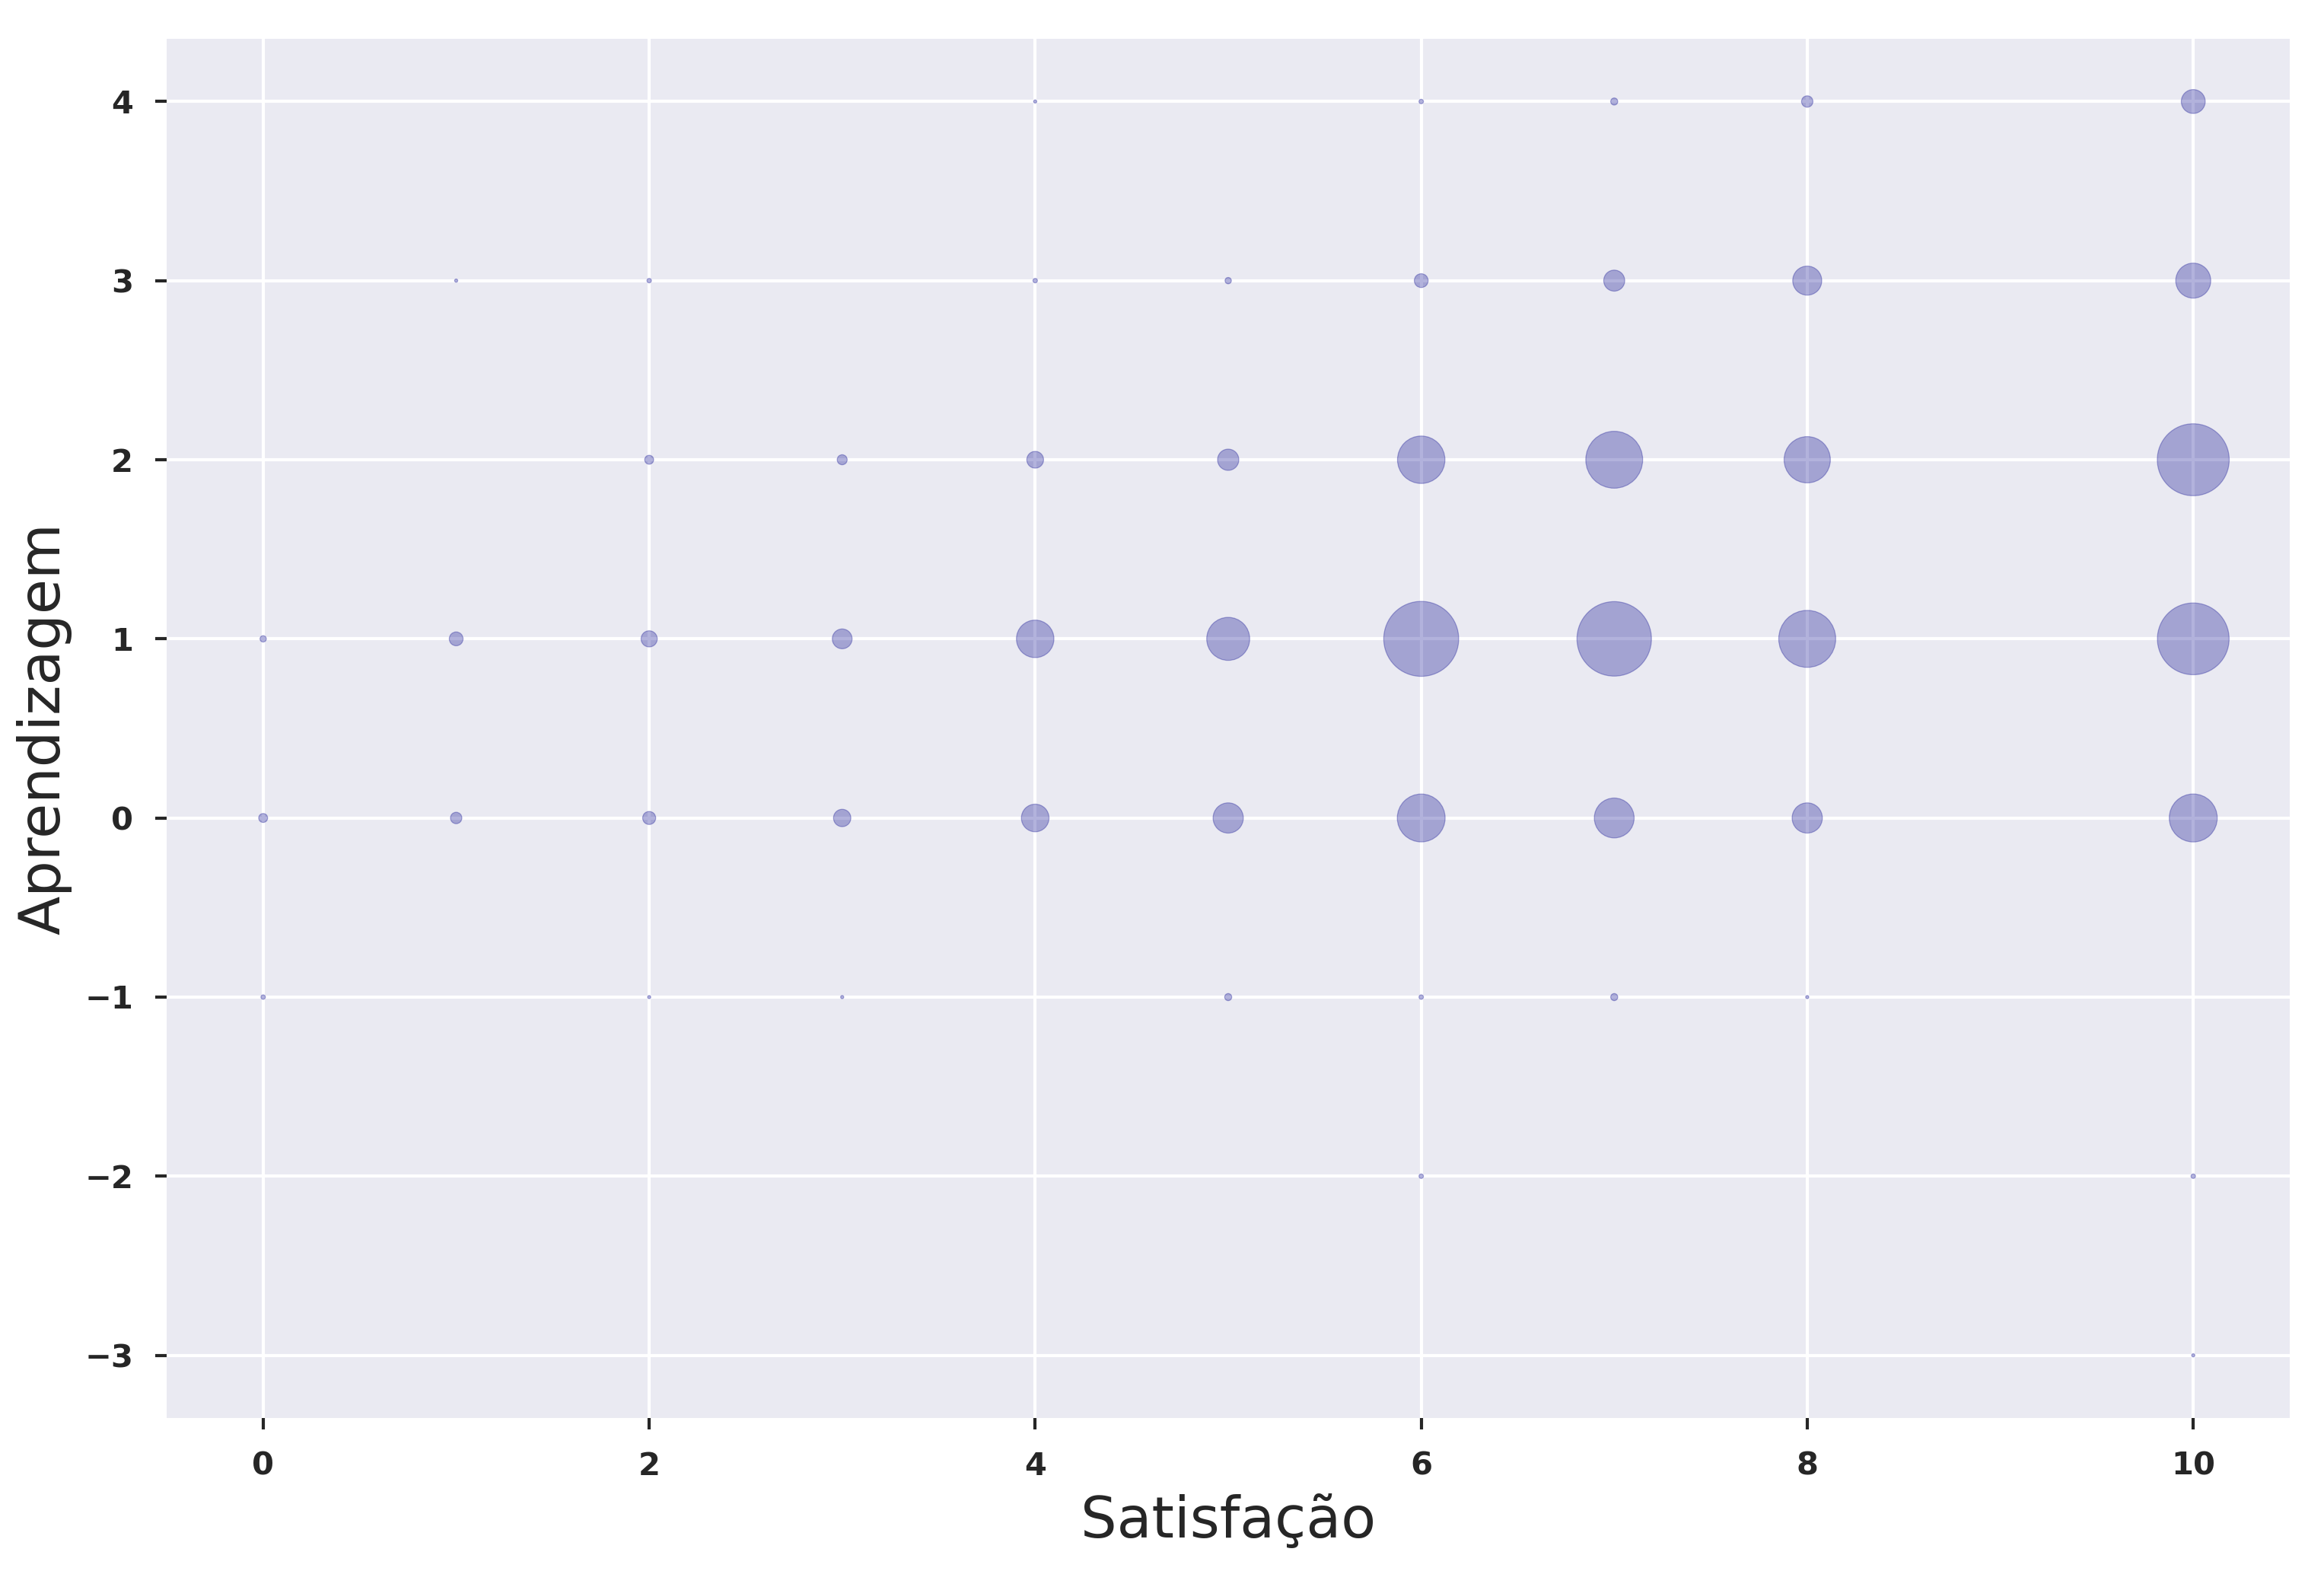
\includegraphics[width=0.5\textwidth]{aprendizagem-vs-satisfacao}

	\caption{\foreign{Bubble-plot} da aprendizagem em função de cada um dos preditores.}
	\label{fig:bubble-plots}
\end{figure}

O modelo de regressão mais simples é o linear.
Porém, uma análise visual dos gráficos de aprendizagem em função de cada um dos preditores não torna evidente qualquer possível relação linear (fig.~\ref{fig:bubble-plots}).
Então experimentamos outros algoritmos de regressão, conforme apresentado na Tabela~\ref{tab:reg-ds-1}.

O conjunto de dados usado para as regressões foi extraído do conjunto completo (Figura~\ref{fig:dataset}), tomando o cuidado de que um dado aluno não estivesse presente mais do que uma vez.
Fizemos esse tratamento com o intuito de evitar correlação entre os exemplos.

Em seguida, aplicamos cada um dos algoritmos a 70\% dos exemplos no conjunto de dados (conjunto de treinamento), explorando sistematicamente o espaço de hiper-parâmetros à procura de um mínimo global no erro quadrático médio da regressão.

O melhor índice de determinação, calculado sobre os 30\% exemplos restantes (conjunto de teste), foi $R^2 \approx 0,193$ para o modelo XGBoost, composto por um conjunto de árvores de decisão simples \cite{Friedman2001}.
Isso significa que nosso melhor modelo é capaz de explicar apenas 19\% das variações na aprendizagem, a partir dos preditores propostos.
Embora seja baixo, podemos argumentar  que a aprendizagem sofre maior influência de outros parâmetros mais importantes, que não temos acesso aqui, como a metodologia de aprendizagem, a qualidade das atividades e conteúdo proposto \etc.

\begin{table}[b]
	\centering
	\caption{Métricas de qualidade dos vários algoritmos de regressão aplicados a DS.}
	\label{tab:reg-ds-1}
	\begin{tabular}{llccc}
		\toprule
		Algoritmo   & Linear? &  RMSE &   MAE & $R^2$\\
		\midrule
		XGBoost  & Não     & 0,769 & 0,581 & \textbf{0,193}\\
		\foreign{Random Forest} & Não & 0,772 & 0,594 & 0,186\\
		Árvore de decisão & Não &  0,775 & 0,596 & 0,181\\
		Adaboost & Não     & 0,806 & 0,629 & 0,113\\
		\foreign{ElasticNet} & Sim & 0,819 & 0,640 & 0,083\\
		SVR & Não & 0,835 & 0,612 & 0,048\\
		\bottomrule
	\end{tabular}
\end{table}

Agora que sabemos que o modelo XGBoost obteve melhor desempenho, podemos experimentar variar os preditores: efetuamos a regressão considerando como preditores as combinações de um, dois e três preditores.
Nesse caso, a métrica mais relevante é o $\bar R^2$, que pondera o índice de determinação pela quantidade de preditores.
Por exemplo, para dois modelos com o mesmo $R^2$, o primeiro com um e o segundo com dois preditores, o melhor modelo é aquele com maior $\bar R^2$.

Os resultados desse experimento estão na Tabela~\ref{tab:r2-adjusted}, ordenados por $R^2$ e $\bar R^2$.
Concluimos que o melhor modelo é de fato o que utiliza todos os três preditores propostos: satisfação, relevância e ritmo.

\begin{table}
	\centering
	\caption{$R^2$ e $\bar R^2$ para o algoritmo XGBoost aplicado a DA e DS.}
	\label{tab:r2-adjusted}
	\begin{tabular}{ccccccc}
		\toprule
		           &            &            & \multicolumn{2}{c}{ Data Science  } & \multicolumn{2}{c}{ Data Analytics }\\
		\midrule
		Relevância & Ritmo      & Satisfação & $R^2$     & $\bar R^2$ & $R^2$     & $\bar R^2$\\
		\midrule
		\checkmark & \checkmark & \checkmark & 0,193 & 0,191 & 0,213 & 0,211 \\
		           & \checkmark & \checkmark & 0,125 & 0,120 & 0,184 & 0,183 \\
		\checkmark &            & \checkmark & 0,115 & 0,114 & 0,147 & 0,146 \\
		           &            & \checkmark & 0,075 & 0,074 & 0,130 & 0,130 \\
		\checkmark & \checkmark &            & 0,071 & 0,070 & 0,096 & 0,095 \\
		\checkmark &            &            & 0,052 & 0,051 & 0,019 & 0,018 \\
		           & \checkmark &            & 0,014 & 0,014 & 0,076 & 0,075 \\
		\bottomrule
	\end{tabular}
\end{table}

A mesma análise pode ser feita para DA, o que nos leva inicialmente à escolha do algoritmo, conforme ilustra a Tabela~\ref{tab:reg-da-1}.
Curiosamente, nesse caso o algoritmo de árvore de decisão obteve melhor desempenho que o \foreign{random forest} (o oposto para DS).
Ainda assim, novamente o melhor (maior $R^2$) algoritmo foi o XGBoost; porém com $R^2$ similar ao caso de DS.

Em seguida variamos os preditores e obtemos os resultados apresentados na Tabela~\ref{tab:r2-adjusted}.
O resultado é similar ao de DS: o modelo que utiliza todos os preditores é melhor.

\begin{table}
	\centering
	\caption{Métricas de qualidade dos vários algoritmos de regressão aplicados a DA.}
	\label{tab:reg-da-1}
	\begin{tabular}{llccc}
		\toprule
		Algoritmo               & Linear? & RMSE  &   MAE & $R^2$\\
		\midrule
		XGBoost                 & Não     & 0,958 & 0,760 & \textbf{0,213}\\
		Árvore de decisão       & Não     & 0,958 & 0,762 & 0,212\\
		\foreign{Random Forest} & Não     & 0,959 & 0,770 & 0,210\\
		Adaboost                & Não     & 0,983 & 0,801 & 0,170\\
		\foreign{ElasticNet}    & Sim     & 0,985 & 0,793 & 0,167\\
		SVR                     & Não     & 0,994 & 0,797 & 0,152\\
		\bottomrule
	\end{tabular}
\end{table}

Resumindo, para DA e DS o melhor modelo XGBoost utilizando os três preditores propostos consegue explicar apenas aproximadamente 20\% das variações observadas (hipótese 3).
Ainda assim, o fato de $R^2$ ser demasiadamente baixo torna essa conclusão duvidosa.




	\section{Conclusão}

Neste trabalho nós avaliamos a influência da expectativa do aluno (de obter um posto de trabalho como cientista de dados) na sua aprendizagem e como isso pode ser incongruente com propostas de adotar currículos baseados em competências e habilidades em cursos livres de ciência de dados.
Avaliamos ainda como a satisfação do aluno com o curso, a relevância percebida por ele sobre os tópicos abordados e o ritmo do curso também infererem na aprendizagem.

Concluimos que nas aulas de ferramentas de ciências de dados os alunos apresentam maior aprendizagem, possivelmente devido à relação explícita delas com os requisitos de vagas de trabalho.
Esse resultado sugere duas estratégias para aprimorar a aprendizagem nas demais aulas: (1) desenvolvê-las utilizando as ferramentas (aprendizagem significativa) e (2) tornando mais evidente a relação dessas aulas com os requisitos do mercado (teoria do valor da expectativa).
Concluimos ainda que efeito análogo \emph{não} acontece para as aulas de algoritmos.

Finalmente, demonstramos o ritmo do curso, a relevância dos tópicos abordados e a satisfação com o curso são capazes de explicar no máximo 20\% da aprendizagem.
Esse resultado é inconclusivo, mas sugere um prosseguimento: decompor a satisfação nas suas componentes, propondo novos experimentos com os alunos.

Outras oportunidades são: mapear os tópicos das aulas para as unidades de conhecimento e áreas de competências estabelecidas pelo DS-BoK \cite{Demchenko2017} e checar as hipóteses 1 e 3 em sub-conjuntos nessas unidades e áreas.


	%-- Referências
	\bibliographystyle{abntex2-alf}
	\bibliography{referencias}

	%-- Apêndices
	\appendix
	\section{\foreign{Reproducible research}}
\label{ap:rr}

A análise de dados apresentada neste trabalho segue princípios de \foreign{reproducible research} \cite{Peng2011}. Isso significa que ela pode ser reproduzida utilizando os arquivos disponibilizados no seguinte repositório Git\footnote{Git (\url{git-scm.com}) é um sistema de versionamento de arquivos.}:

\begin{center}
	\url{http://github.com/irpagnossin/tcc-cae-icmc-usp}
\end{center}

Além disso, esse artigo foi criado com \LaTeX, cujos arquivos-fonte também podem ser acessados no repositório acima.

\end{document}


Problema de pesquisa: definição e aplicação de currículo baseado em competências para DS
Objetivo geral: adotar currículo baseado em competências para DS
Objetivo específicos:
- Averiguar a receptividade de currículos baseado em competências (medida: aprendizagem percebida).